\documentclass[12pt,b5paper]{report}
\usepackage[margin=1in]{geometry}
\usepackage[pdftex]{graphicx} %for embedding images
\usepackage{url} %for proper url entries
\usepackage[bookmarks, colorlinks=false, pdfborder={0 0 0}, pdftitle={<pdf title here>}, pdfauthor={<author's name here>}, pdfsubject={<subject here>}, pdfkeywords={<keywords here>}]{hyperref} %for creating links in the pdf version and other additional pdf attributes, no effect on the printed document

\usepackage{fancyhdr}

\usepackage{fancyvrb}
\usepackage{color}
\usepackage[utf8]{inputenc}
\usepackage{float}

\usepackage{pst-node}% http://ctan.org/pkg/pstricks
\usepackage{xcolor}% http://ctan.org/pkg/xcolor
\usepackage{eso-pic}% http://ctan.org/pkg/eso-pic
\usepackage{lipsum}% http://ctan.org/pkg/lipsum

\usepackage{tikz}
\usetikzlibrary{calc}
\newcommand\HRule{\rule{\textwidth}{1pt}}

\usepackage{titlesec}

% break lines in code
\usepackage{spverbatim}

% remove this to get back to the old chapter style
% \titleformat{\chapter}[block]
%   {\normalfont\huge\bfseries}{\thechapter.}{1em}{\Huge\vspace{1em}}
% \titlespacing*{\chapter}{0pt}{-19pt}{0pt}

%\usepackage[final]{pdfpages} %for embedding another pdf, remove if not required

\begin{document}
\renewcommand\bibname{References} %Renames "Bibliography" to "References" on ref page

% remove page numbering
\pagenumbering{gobble}

%include other pages
\topskip0pt
\vspace*{\fill}

\begin{center}
\Large
Mini Project Report

\hspace{0.7em}

on

\hspace{0.7em}

\Large{\bfseries{BRIDGE}}

\normalsize
Student Self Monitoring System

\hspace{1em}

submitted by

\hspace{1em}

\large
Abin Simon ( 12150005 )

\large
Aayisha A A ( 12150076 )

\large
Abhai Kollara ( 12150002 )

\hspace{1em}

\normalsize
In partial fulfilment of the requirements for the award of degree of Bachelor of Technology in Computer Science and Engineering.

\hspace{1em}

\large
DIVISION OF COMPUTER ENGINEERING

SCHOOL OF ENGINEERING

\hspace{1em}

COCHIN UNIVERSITY OF SCIENCE AND TECHNOLOGY

\hspace{1em}

\normalsize
MARCH 2017
\end{center}

\vspace*{\fill}

\newpage
\begin{tikzpicture}[remember picture, overlay]
  \draw[line width = 4pt] ($(current page.north west) + (0.5in,-0.5in)$) rectangle ($(current page.south east) + (-0.5in,0.5in)$);
\end{tikzpicture}

\topskip0pt
\vspace*{\fill}

\begin{center}

\large
DIVISION OF COMPUTER ENGINEERING\\
SCHOOL OF ENGINEERING\\

\hspace{1em}

COCHIN UNIVERSITY OF SCIENCE AND TECHNOLOGY\\

\hspace{1em}

\emph{\LARGE Certificate}

\hspace{1em}

\normalsize
Certified that this is a bonafide record of the Minor Project titled

\hspace{1em}

\Large{\bfseries{BRIDGE}}

\normalsize
Student Self Monitoring System

\hspace{1em}

done by

\hspace{1em}

\large
Abin Simon ( 12150005 )

\large
Aayisha A A ( 12150076 )

\large
Abhai Kollara ( 12150002 )

\hspace{1em}

\normalsize
of VI Semester, Computer Science and Engineering in the year 2017 in partial fulfillment requirements for the award of degree of Bachelor of Technology in Computer Science and Engineering of Cochin University of Science and Technology.

\hspace{1em}
\vspace{5em}

\begin{minipage}[b]{0.33333\textwidth}
\raggedright
Ancy Zachariah

Head of Division\\
\end{minipage}%
\begin{minipage}[b]{0.33333\textwidth}
\centering
Pramod Pavithran / Damodaran.V

Project Coordinator\\
\end{minipage}%
\begin{minipage}[b]{0.33333\textwidth}
\raggedleft
Anu M.

Project Guide\\
\end{minipage}

\end{center}

\vspace*{\fill}

\newpage
\vspace{2in}

\LARGE{\bfseries{Acknowledgement}}

\hspace{1in}

\normalsize
We take this opportunity to express our profound gratitude and deep regards to our guide \textbf{Mrs Anu M.}
,for providing us with the right guidance and advice at the crucial junctures and for her constant encouragement throughout the course of this project. We are highly indebted to \textbf{Asst. Prof. Pramod Pavithran}
 and \textbf{Mr Damodaran.V}
 , Division of Computer Science our batch coordinator for her constant supervision and support for completing the project. We extend our sincere thanks to our respected Head of the department, \textbf{Ancy Zachariah}
 ,Head of Division,Division of Computer Science and all other faculty members of for sharing their valuable time and knowledge with us. We thank God, the almighty for blessing us with his grace and taking our endeavour to a successful culmination. Lastly we would like to thank my friends and family for their constant encouragement without which this project would not have been possible.

\begin{flushright}

\vspace{2em}

Thanking you,\\
\vspace{1em}

Abin Simon\\
Aayisha A A\\
Abhai Kollara\\

\end{flushright}

% \newpage
% \vspace{2in}

\LARGE{\bfseries{Decleration}}

\hspace{1in}

\normalsize
We, Miss Aayisha A A,Mr Abhai Kollara Dilip,Mr Abin Simon hereby declare that this project is the record of authentic work carried out by us during the academic year 2016 -2017 and has not been submitted to any other University or Institute towards the award of any degree.

\vspace{5em}

\begin{minipage}[b]{0.33333\textwidth}
\raggedright
Abin Simon
\end{minipage}%
\begin{minipage}[b]{0.33333\textwidth}
\centering
Aayisha A A
\end{minipage}%
\begin{minipage}[b]{0.33333\textwidth}
\raggedleft
Abhai Kollara
\end{minipage}

\newpage
\vspace{2in}

\centerline{\large{\bfseries{ABSTRACT}}}

\hspace{1in}

\normalsize
We are living in an age where the art of technology and the art of teaching has come a long way. With bridge we intent to interlace those by helping to bridge the communication gap between teachers and students. Currently, even though teachers use technology to reach out to students the solutions are more or less ad-hoc. The communication is spread over different channels, sometimes a phone call, sometimes a text message, and sometimes nothing at all. There lacks an efficient way for teachers to communicate to students directly as a group or individually. Also there is no easy way for the students and teachers to keep track of the tasks they have in hand. It is at times really hard for teachers to reach students most of time and they end up relying on the class representative to deliver the message which in itself is not bad, but is less efficient.

Bridge intents to solve all the above stated problems by implementing a application using which the teachers and students can communicate seamlessly with each other, keep track of everything that they have to do, get replies asap and just about anything that helps make the student teacher communication much more effective and easy.
% In here we will have ways in which
% \begin{itemize}
% \item Teachers will be able to post all details about assignments and schedule exams to a common calender which will be visible to the respective students at any time.
% \item Teachers can also publish any results as well as remarks about a student or a group.
% \end{itemize}
% Now, for students

% \begin{itemize}
% \item They can always see what is coming up next in their calender
% \item They can have a place to update their attendance
% \item They can note down notes of each class and view them later
% \item They can catch up the upcoming events
% \end{itemize}


\pagenumbering{roman} %numbering before main content starts
\tableofcontents
\listoffigures

\pagestyle{fancy}
\fancyhf{}
\rhead{Bridge}
\lhead{}
\rfoot{Page \thepage}
\lfoot{Department of Computer Science and Engineering}

\newpage
\pagenumbering{arabic} %reset numbering to normal for the main content

\chapter{Introduction}

\vspace{1em}
The most important aspect of a academic studies for a student is the involvement of the teachers in the matters of the students. It is also very vital for the student to stay updated about what is happening in the college. With this project we aim to do just that. We are creating a platform that can help the students to easily stay up to date on what is happening in their academic matters. They have an easy and intuitive way to see what is in their calendar.\\

\vspace{1em}
Our platform also provides an effective way for the student to track his daily activities at the academic institute by giving then a simple and efficient platform to take notes and track their attendance. This, we think is a great tool that will help the student of the academic institution to be able to track his time at the institution.\\

\vspace{1em}
The platform with its ability to take down notes for the classes they are attending in the university, in a platform that has their timetable and other data integrated along with it is a huge bonus for the student as it gives them a seamless way to take down notes for a specific period and let them filter it and get all the dada beautifully presented to them which is a huge bonus for a student.

\chapter{System Analysis}

\section{Existing system}

The present system is ineffective in maintaining a student centric model. It mainly consisted of web applications and very few mobile applications. The traditional way of maintaining record is time consuming, not easily accessible ,requires a computer, less user friendly, and laborious.\\

Apart from these all the system we have currently are mostly teacher centric which leads to a hard time for the students to navigate and find what they need.\\

Here are some disadvantages of existing system:
\begin{itemize}
\item Time consuming
\item Not easily accessible
\item Teacher centric
\item Less student friendly
\item Laborious
\end{itemize}

\section{Proposed system}

With our solution we are aiming to provide a simple and intuitive interface for the student. We are also looking forward to provide a student centric model in which the student will able to track his classes at the university.\\

Once the user get registered through their google sign in (which makes the signin and verification process efficient and easy ). The user will be provided with a popup menu in which they could select their respective division head and to which course they are enrolled to.after the completion of sign in process, we will have a wide range of options which include attendance tracking system, notes adding, which could include lecture videos, images and much more feature which make learning easier, it tend to have an added feature of upcoming events which help to clear the backlogs and make the work as timid and as clean as possible\\

\begin{itemize}
\item This system is developed in such a way that even a naive user can also operate the system easily.
\item This system is also secure as the database is managed only by
the administrator of the system.
\item It has an error free verification mechanism
\item Easy way of accessing records and tracking attendance
\end{itemize}


\chapter{System Study}
\section{Software Requirement Specification}

\subsection{Introduction}

\subsubsection{Purpose}
The purpose of this document is to present a detailed description of the Web Publishing System. It will explain the purpose and features of the system, the interfaces of the system, what the system will do, the constraints under which it must operate and how the system will react to external stimuli.

\subsubsection{Intended Audience and Reading Suggestions}
This document is intended for the understanding of complete functionalities that will be provided by the software. Therefore it may be used by anyone who wishes to further develop this software or anyone who intends to understand the full capabilities of the system.

\subsubsection{Scope of the Project}
The software system will be a Student Self Monitoring System intended for the use by students of a college. It is designed so as to help students keep track of their academic activities in college. We include attendance tracking, tasks tracking, notes feature etc for increasing the productivity of students. The attendence tracking mechanism is an extremely useful tool. The notes features allow students to save notes for each period of a day. The feature also supports markdown text which allows the student to go beyond plaintext for their notes.

It is also intended to to minimize the difficulties of communication between students and college authorites which would otherwise have to be performed manually by phone calls or class representatives. More specifically the system allows teachers to notify the students about upcoming tasks/events increasing the efficiency of communication.

The system also contains a relational database containing Students, Teacher, Departments, Classes, Subjects, Notes, Events.

\subsubsection{References}
IEEE. IEEE Std 830-1998 IEEE Recommended Practice for Software Requirements Specifications. IEEE Computer Society, 1998.

Django Official Documentation

\subsubsection{Overview of Document}
The next chapter, the Overall Description section, of this document gives an overview of the functionality of the product. It describes the informal requirements and is used to establish a context for the technical requirements specification in the next chapter.

The third chapter, Requirements Specification section, of this document is written primarily for the developers and describes in technical terms the details of the functionality of the product. 

Both sections of the document describe the same software product in its entirety, but are intended for different audiences and thus use different language.

\subsection{Overall Description}

\subsubsection{Product Perspective}
The software is designed to be a stand-alone web application that is designed to provide a different approach to current learning management systems like Moodle.

\subsubsection{Product Functions}
The primary functions of the software are:
\begin{itemize}
\item Let the students store notes of every period
\item Let the students store and track their attendence of every period
\item Let teachers/admins create and assign events to classes
\item Let students view upcoming classes
\end{itemize}

\subsubsection{User Classes}
The Student Self Monitoring System has two main actors, the user (Student) and the admin (Teachers/other authorities). The role of the admin is to provide the system with sufficient data about each classes, subjects, departments and teachers involved. The admin has near complete access to the database. It is also the role of the admin(teacher) to add upcoming events/tasks to the software system.

\subsubsection{Operating Environment}
The software is designed to be platform independent and to work on any major web browser that supports Javascript. The software is also designed resposively so as to run on mobile web browsers.

\subsubsection{Design and Implementation Constraints}
The major design constraint was to implement the software to run on mobile platforms. The UI should be designed responsively to accomodate mobile view

\subsubsection{Assumptions and Dependencies}
The software requires a server that supports running Django 1.11 on Python 2.7

\subsection{External Interface Requirements}

\subsubsection{User Interface}
The UI must be responsive and must view correctly on mobile views. The UI is intended to be platform independent ie it should be the same irrespective of the OS and web browser. A material design is applied thorought the application

\subsubsection{Hardware Interfaces}
From client side, devices with at least 512 MB of RAM is recommended along with a low latency high bandwidth internet connectivity. This is applicable for both desktop and mobile systems.

\subsubsection{Software Interfaces}
The software communicates with a MySQL database through the Django interface. Basic built-in python libraries are assumed available. 

The software also accesses the Google sign-in API for secure login.

\subsection{System Features}

This section outlines the use cases for each of the actors seperately; the user and the admin.

\subsubsection{Admin Use Case}

\begin{itemize}

\item The admin must be able to add/remove data to/from the following entities : 

\begin{itemize}
\item Departments
\item Teachers
\item Subjects
\item Classes
\end{itemize}

\item The admin must also be able to specify the relation between teacher, subject and classes.

\item The admin must be able to add new events to the upcoming event list for the users to view

\end{itemize}

\subsubsection{User Use Case}

\begin{itemize}

\item Login – User must be able to login using Google Accounts
\item User must be allowed to pick a class of his choice
\item Attendance Tracking

\begin{itemize}
\item The user must be able to view the current attendance
\item The user must be update the attendace on a daily basis
\end{itemize}

\item Notes

\begin{itemize}
\item User must be able to save notes for every period in a day
\item Markdown text should be supported
\item Images should be supported
\item User must be able to view all the notes saved as of yet
\end{itemize}

\item Upcoming Events

\begin{itemize}
\item User must be able to view upcoming events that are added by admins
\item User must have a calender view of upcoming events
\end{itemize}

\end{itemize}

\subsection{Other Non-Functional Requirements}

\subsubsection{Safety Requirements}
Logins must be completely secure and only admins must be allowed to access administrator interfaces.

\section{Hardware and Software Requirements}

\subsection{Hardware specification}
\vspace{1em}
\begin{itemize}
\item RAM: Recommended 512MB or above
\item Storage: 10 GB or above
\item Connectivity: Low latency internet with high bandwidth
\end{itemize}
\subsection{Software specification}
\begin{itemize}
\item OS: Windows, OSX, or Linux ( or any unix system )
\item Env: Python 2.x
\item Database: MySQL
\item Web browser ( preferable Chrome or Firefox )
\end{itemize}


\chapter{System Design}

\section{Data Flow Diagrams}

The dfd \ref{fig:dfd1} below show in the higer level data flow in the project

\vspace{1em}

\begin{figure}[H]
\centering
\includegraphics[height=3in, clip=true]{./dfd1}
\caption{First level dfd}
\label{fig:dfd1}
\end{figure}

\vspace{1em}

This dfd \ref{fig:dfd2} shows how the project handles data within

\vspace{1em}

\begin{figure}[H]
\centering
\includegraphics[height=5in, clip=true]{./dfd2}
\caption{Inner dfd}
\label{fig:dfd2}
\end{figure}


% \vspace{1in}  % to deal with image overlap issues
% \mbox{}
\newpage

\section{Modular Design}

\subsection{Login}
This module handles the user authentication and login.
The component is dependent on Google login for its authentication, as we leverage Google signin module to make the tradition of the user into our app much more easier and faster.

Initially when the user logs into the application is when we create an account for them and register them. When the user logs into the application, we get the user to login to their Google account and we can use the Google API top get the user details like user-id, name, email, profile-image etc. This makes it easer for the user as do not have to manually add in their name or profile image. Only thing they will have to manually set is which class they are studying in.

Now from the next time the user logs in, we will directly log them into their account ready to go.

\subsection{Landing Page}
The landing page is the most important and most viewed part of the whole application. It encompasses details a user would probably need at that time like upcoming events, which data about the class that is currently going on. It also lets them take down notes which they can later view using the notes module.

For each subject of the day we provide the name of the teacher, time of the class, etc which helps the student to plan for their class.
The place provided to jot down notes for the subject also helps them to take down notes during the classes which will be really useful for them for later reference.

\subsection{Notes}
Notes module is aimed at providing an interface for the student( user ) to view all the notes they have taken in the class and go through them.
It is a very useful and powerful utility at the end of a semester as it will let them view all the notes they have in one place and go through them quickly and efficiently.

You can also use the notes view to filter your notes based on the date or the subject which is a really simple but powerful way to summarize a whole semester.

\subsection{Attendance}
One another very important module is the Attendance module which lets the student track their attendance for each subject they have. The student on attending or net attending a specific subject class can update their attendance using the attendance module. All the user data is saved in real-time with the backed and they will be able to check their any time.

The per subject nature of the attendance module also helps them to know which subjects they have missed the most and concentrate on them individually.

\subsection{Calendar}
The Calendar module is used to view the overview of all the events. It shows you all the events and submissions you have for the future. While the upcoming events module only shows you the close and upcoming events, in the calendar module we can see all the upcoming events in the future.

It has a normal calender like intercase with events listed under the specific dates which makes it much more intuitive and easy.


\chapter{System Implementation}

\section{Sample Code}

\subsection{Sample view handlers}
A view handler is a methood which is a specification in django which handles a http request and makes the response.

\input{./handler.tex}

\subsection{Url defenitions}
These define the endpoints fot the backend api

\input{./urls.tex}

\subsection{Model defenitions}
These contains the database models for the project

\input{./models.tex}

\subsection{Base html template}
A basic html template for a page

\input{./index.tex}

\subsection{Sample module in js}
Our js file in a modular design and the below show is the code to initialize a user account.

\input{./script.tex}

\subsection{Sample CSS file}
In here we define the styling for the elements

\input{./style.tex}



\section{Screenshots}

\begin{figure}[htb]
    \centering
    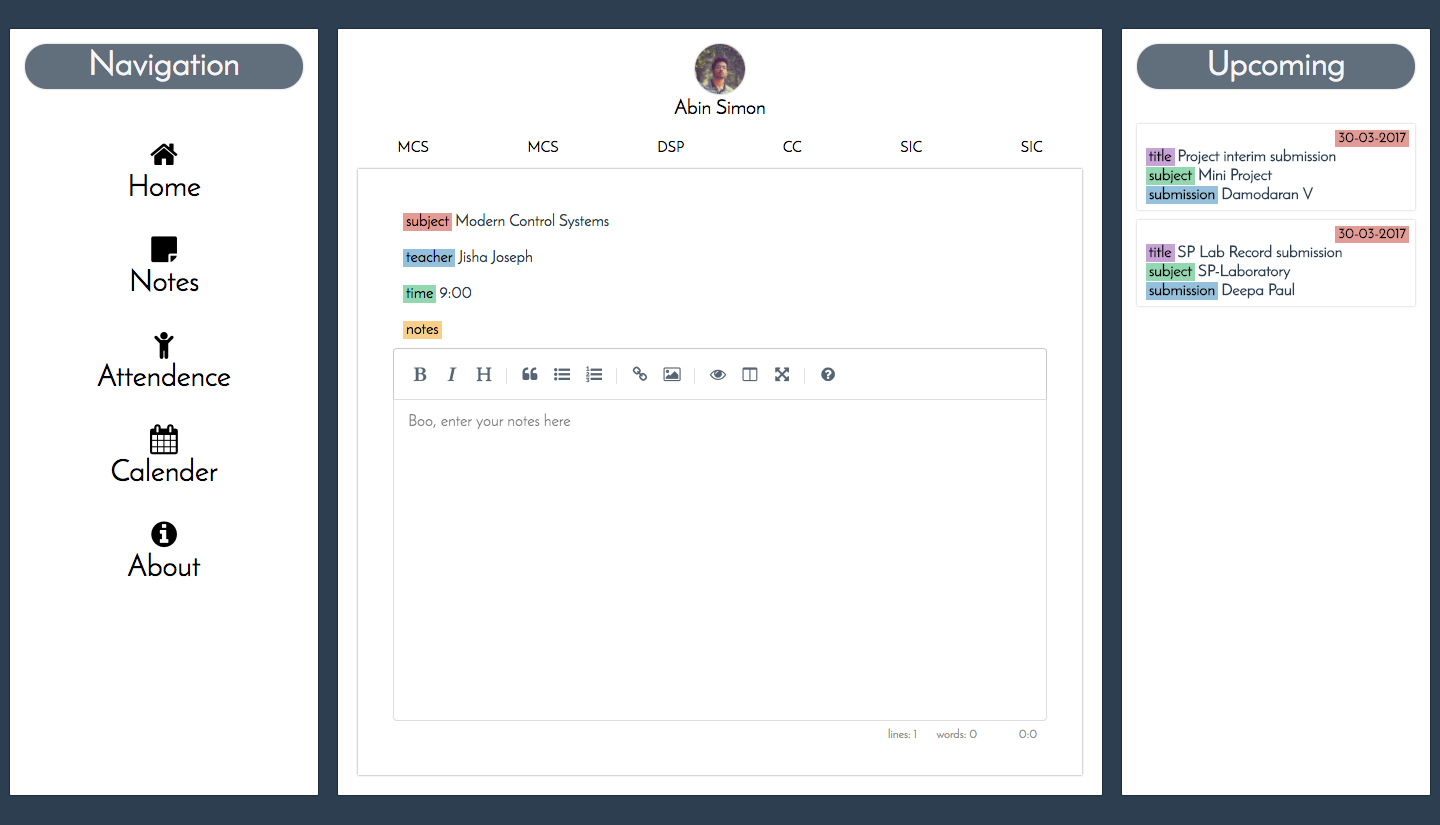
\includegraphics[width=\linewidth]{landingpage.png}
    \caption{Landing page}
    \label{fig:landingpage} % insert suitable label, this is used to refer to a fig from within the text as shown above
\end{figure}

\begin{figure}[htb]
    \centering
    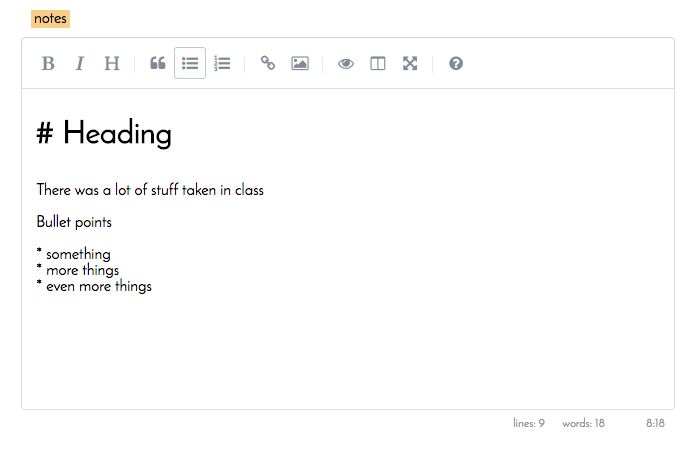
\includegraphics[width=\linewidth]{notesmd.png}
    \caption{Write notes in markdown}
    \label{fig:notesmd} % insert suitable label, this is used to refer to a fig from within the text as shown above
\end{figure}

\begin{figure}[htb]
    \centering
    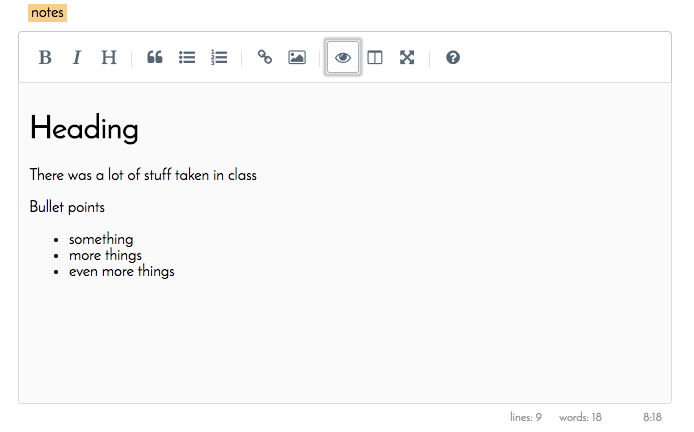
\includegraphics[width=\linewidth]{notescompiled.png}
    \caption{Compiled the written notes to actual contet in place}
    \label{fig:notescompiled} % insert suitable label, this is used to refer to a fig from within the text as shown above
\end{figure}

\begin{figure}[htb]
    \centering
    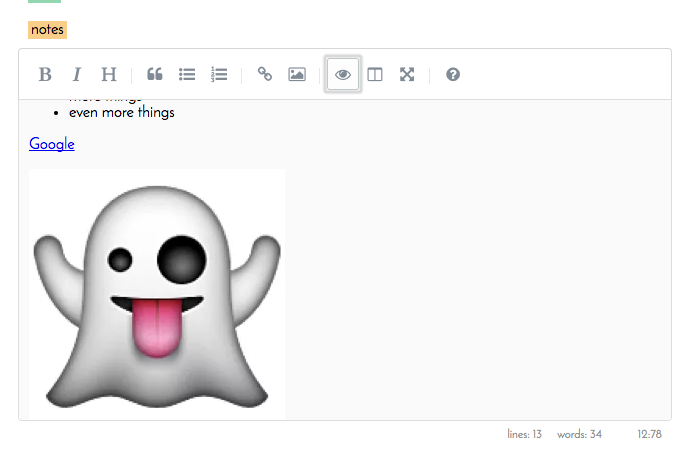
\includegraphics[width=\linewidth]{noteswithimages.png}
    \caption{You can even have notes with images and links}
    \label{fig:noteswithimages} % insert suitable label, this is used to refer to a fig from within the text as shown above
\end{figure}

\begin{figure}[htb]
    \centering
    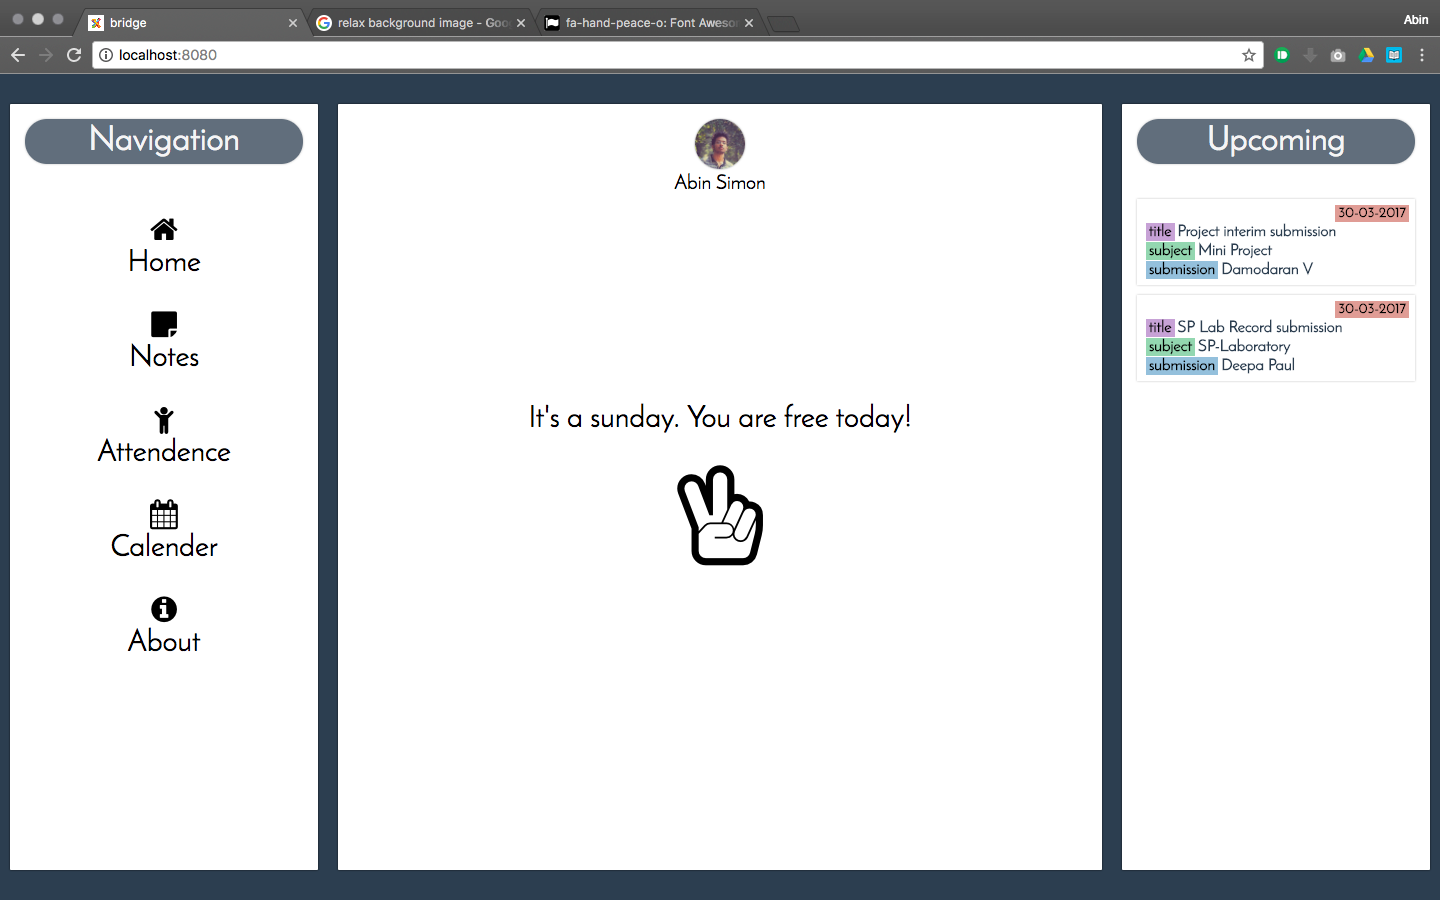
\includegraphics[width=\linewidth]{holiday.png}
    \caption{You can even have notes with images and links}
    \label{fig:holiday} % insert suitable label, this is used to refer to a fig from within the text as shown above
\end{figure}

\begin{figure}[htb]
    \centering
    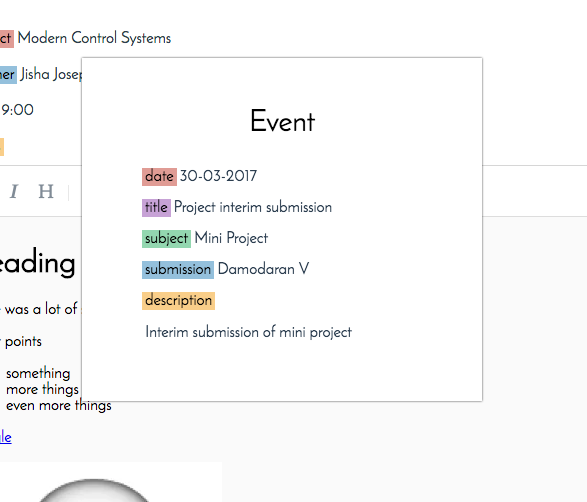
\includegraphics[width=\linewidth]{eventinfo.png}
    \caption{Detailed information about upcoming events}
    \label{fig:eventinfo} % insert suitable label, this is used to refer to a fig from within the text as shown above
\end{figure}

\begin{figure}[htb]
    \centering
    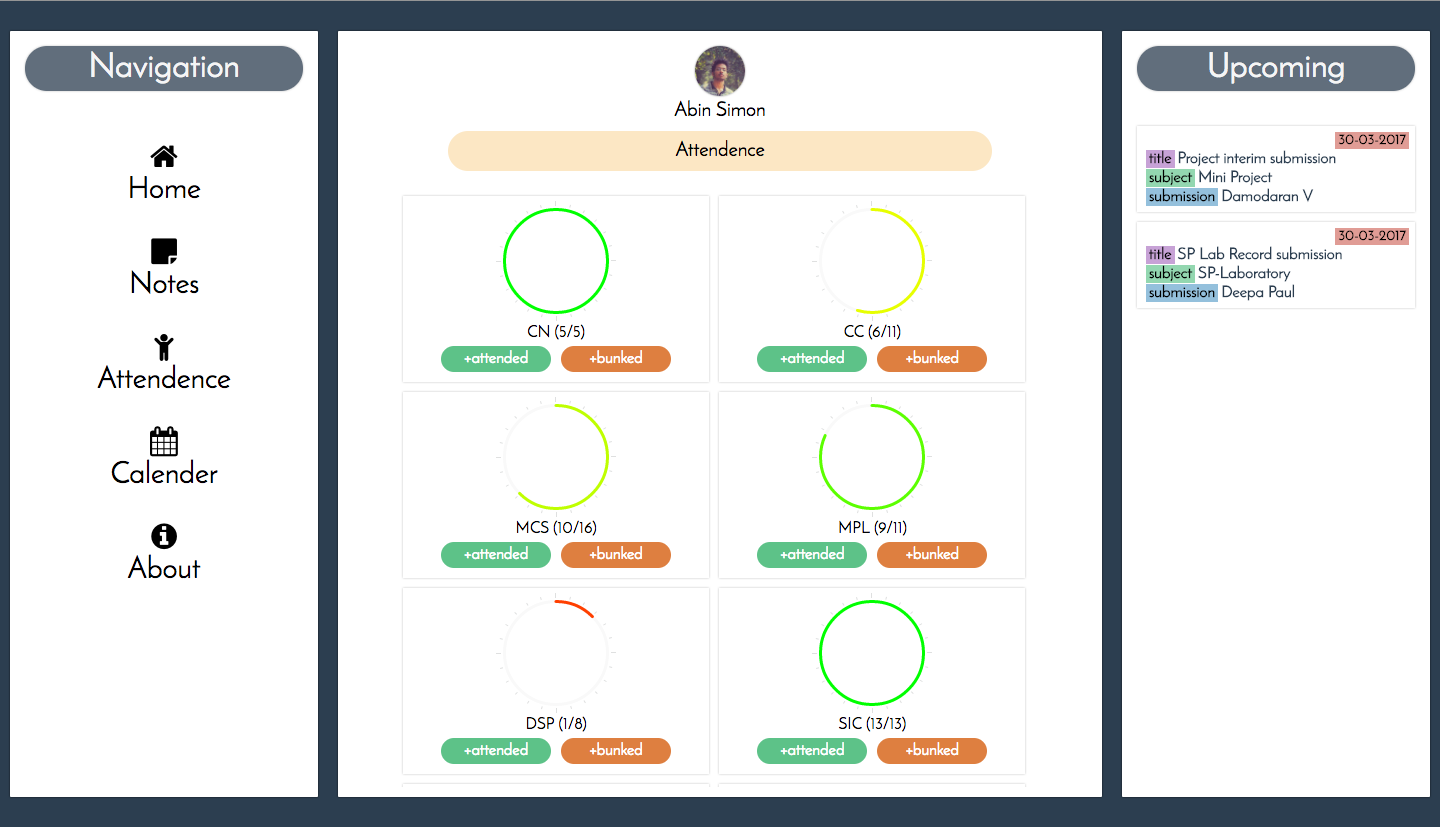
\includegraphics[width=\linewidth]{attendance.png}
    \caption{View and update attendace}
    \label{fig:attendance} % insert suitable label, this is used to refer to a fig from within the text as shown above
\end{figure}

\begin{figure}[htb]
    \centering
    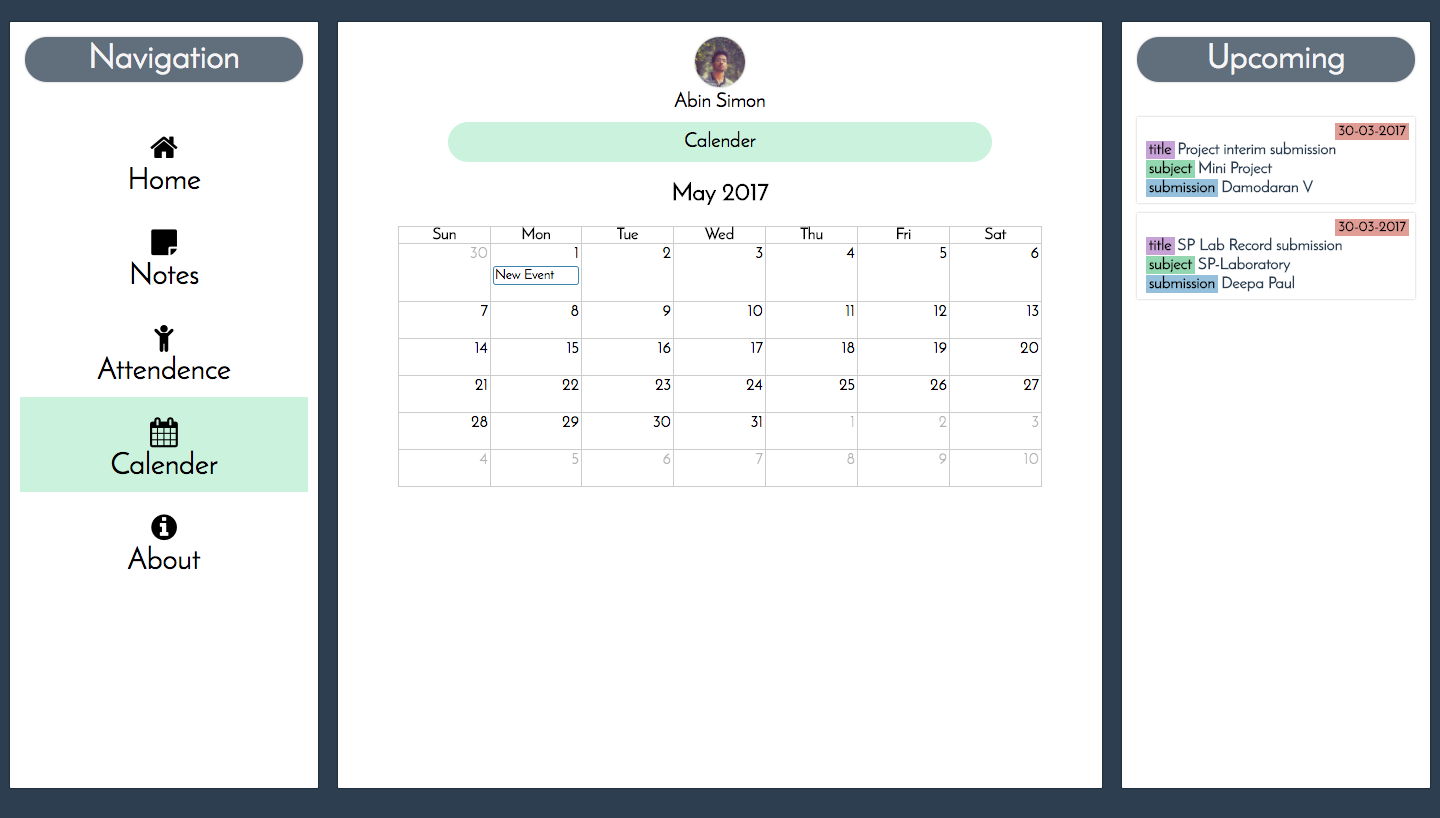
\includegraphics[width=\linewidth]{calendar.png}
    \caption{Calendar entries for events}
    \label{fig:calendar} % insert suitable label, this is used to refer to a fig from within the text as shown above
\end{figure}

\begin{figure}[htb]
    \centering
    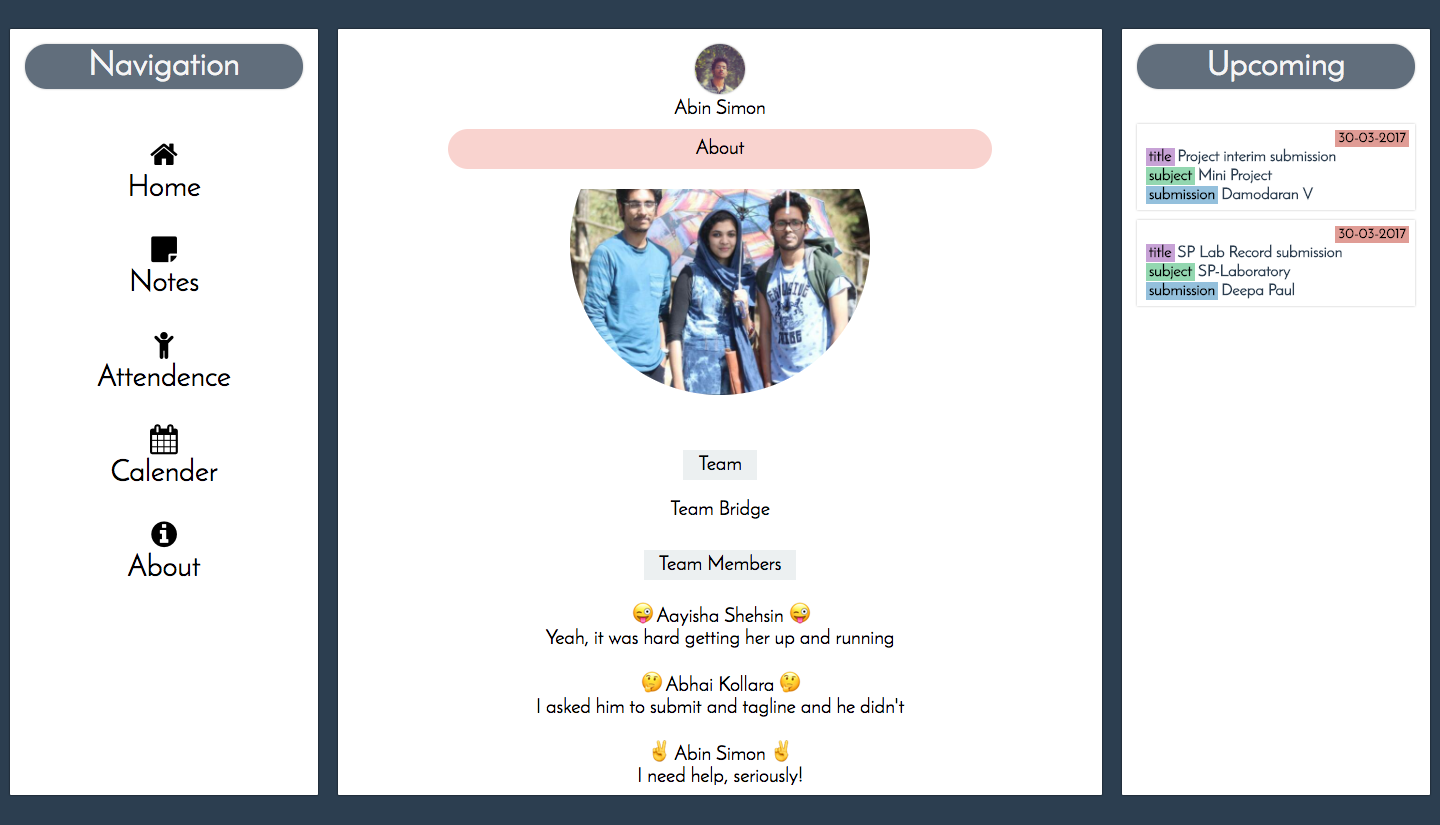
\includegraphics[width=\linewidth]{aboutpage.png}
    \caption{About page}
    \label{fig:aboutpage} % insert suitable label, this is used to refer to a fig from within the text as shown above
\end{figure}

\begin{figure}[htb]
    \centering
    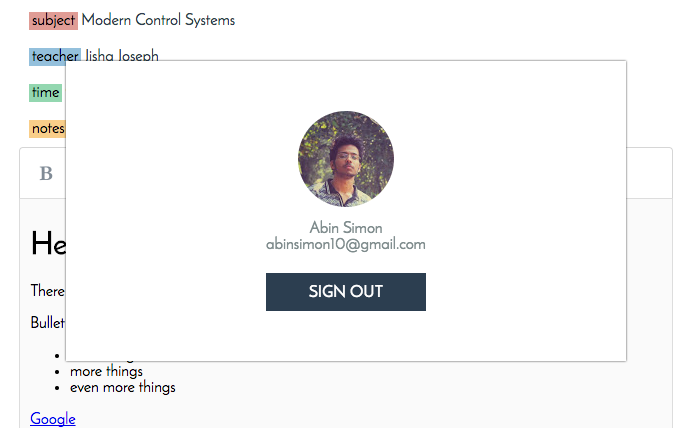
\includegraphics[width=\linewidth]{signoutpopup.png}
    \caption{Popup to sign out of the system}
    \label{fig:signoutpopup} % insert suitable label, this is used to refer to a fig from within the text as shown above
\end{figure}

\begin{figure}[htb]
    \centering
    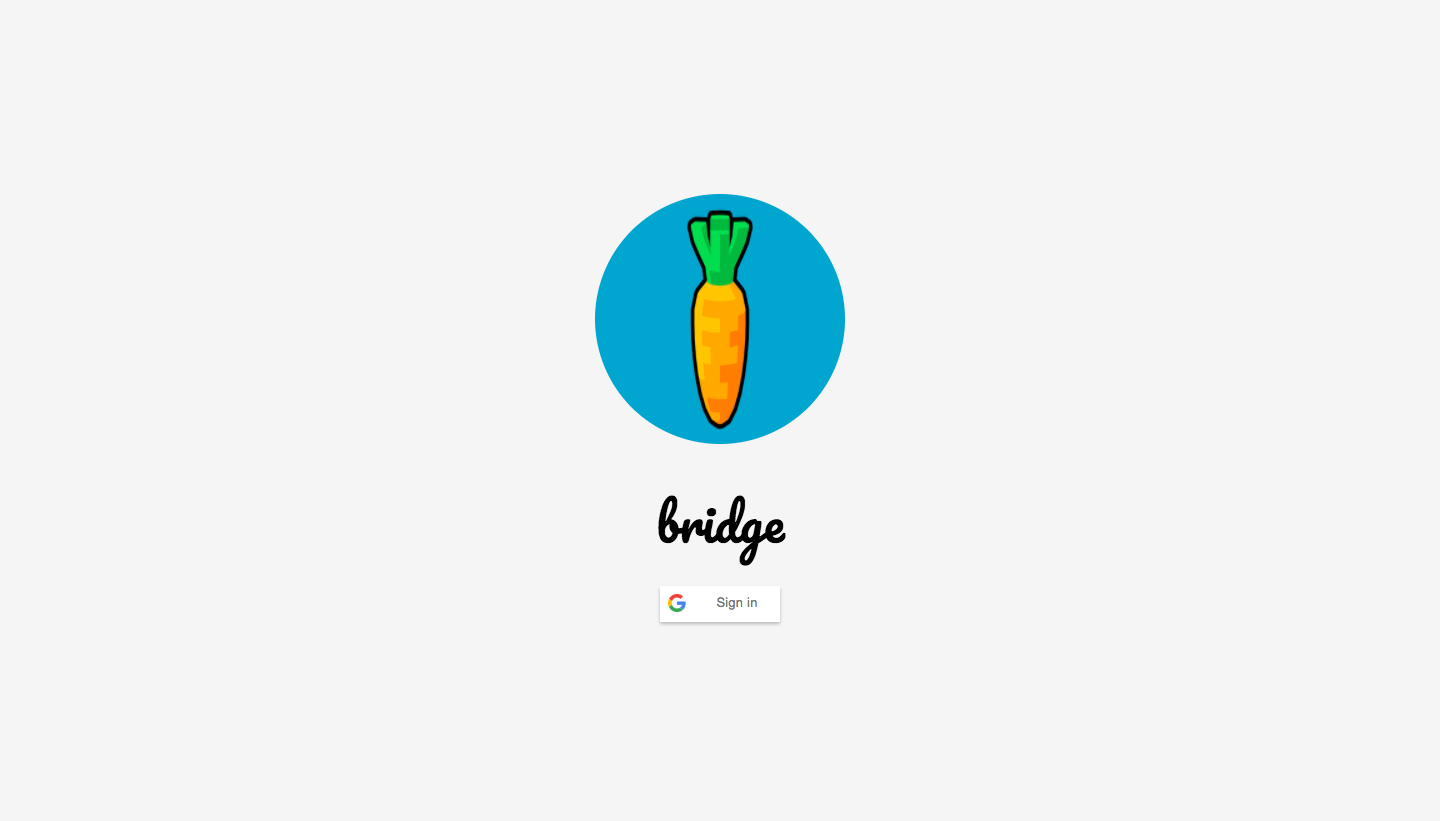
\includegraphics[width=\linewidth]{loginpopup.png}
    \caption{Interface for loggin into the app}
    \label{fig:loginpopup} % insert suitable label, this is used to refer to a fig from within the text as shown above
\end{figure}

\begin{figure}[htb]
    \centering
    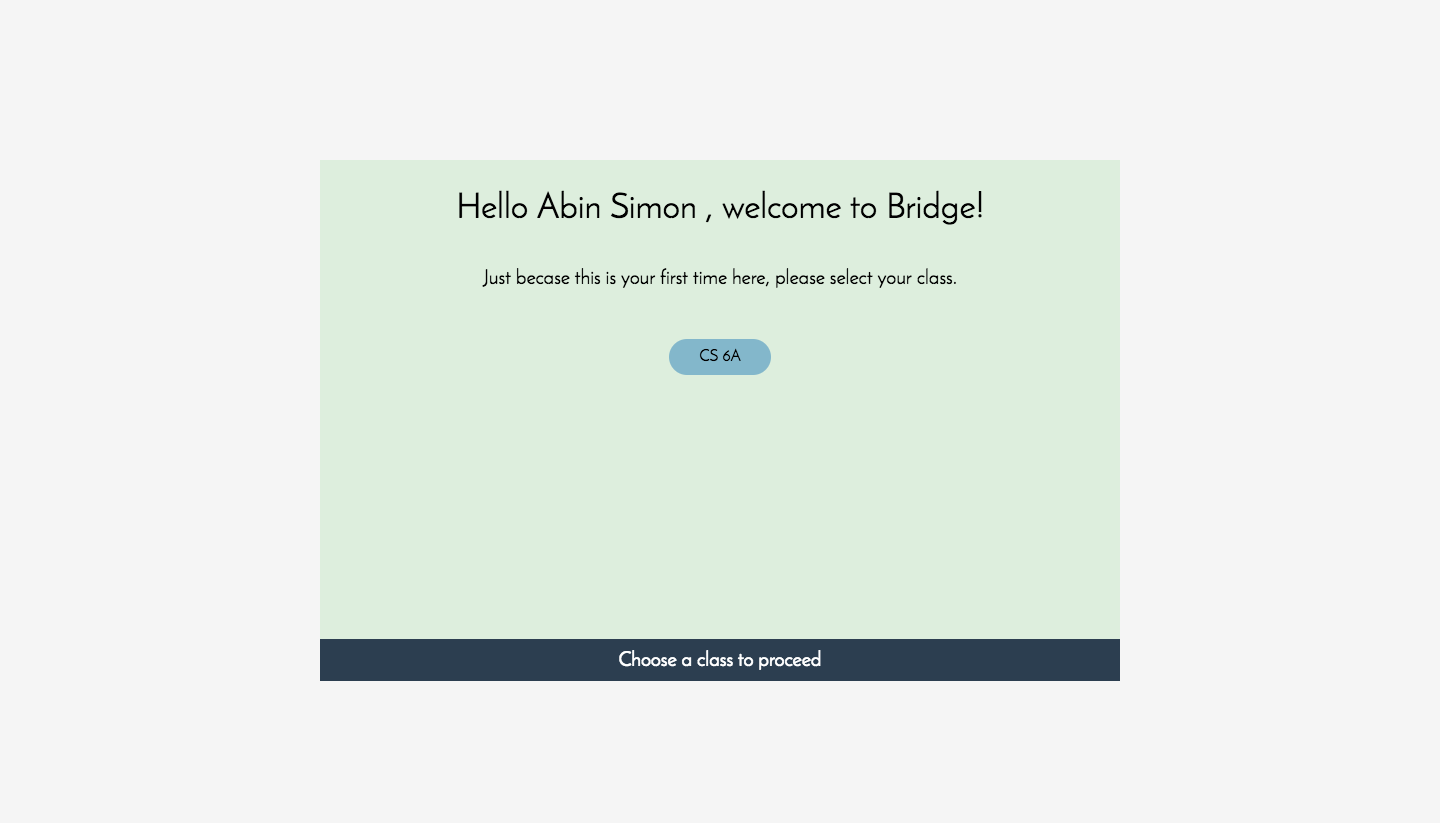
\includegraphics[width=\linewidth]{newuserpopup.png}
    \caption{Interface if the user is a new one so that he can choose a class}
    \label{fig:newuserpopup} % insert suitable label, this is used to refer to a fig from within the text as shown above
\end{figure}

\begin{figure}[htb]
    \centering
    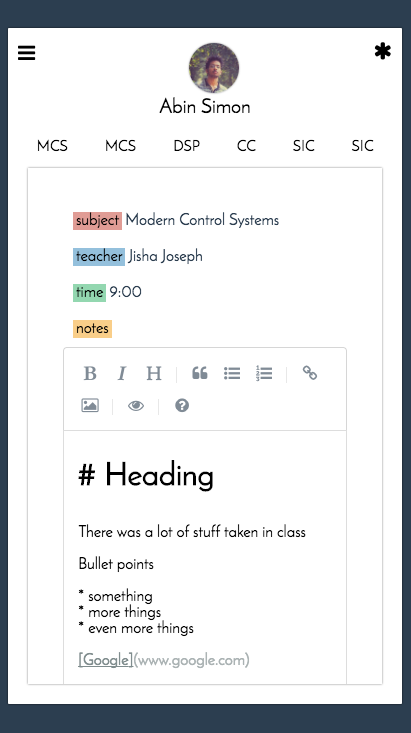
\includegraphics[width=3in]{mobilelanding.png}
    \caption{Landing page on mobile}
    \label{fig:mobilelanding} % insert suitable label, this is used to refer to a fig from within the text as shown above
\end{figure}

\begin{figure}[htb]
    \centering
    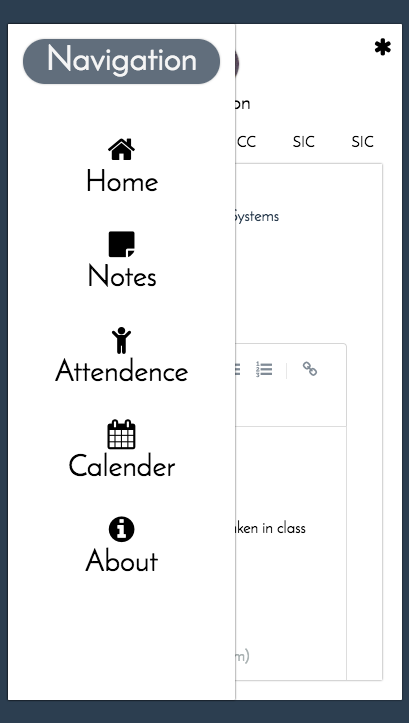
\includegraphics[width=3in]{mobilenav.png}
    \caption{Navigation pane on mobile}
    \label{fig:mobilenav} % insert suitable label, this is used to refer to a fig from within the text as shown above
\end{figure}

\begin{figure}[htb]
    \centering
    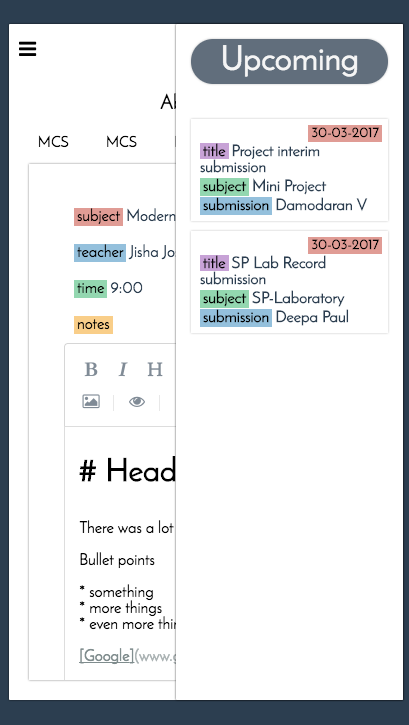
\includegraphics[width=3in]{mobileupcoming.png}
    \caption{Upcoming event display on mobile}
    \label{fig:mobileupcoming} % insert suitable label, this is used to refer to a fig from within the text as shown above
\end{figure}

\begin{figure}[htb]
    \centering
    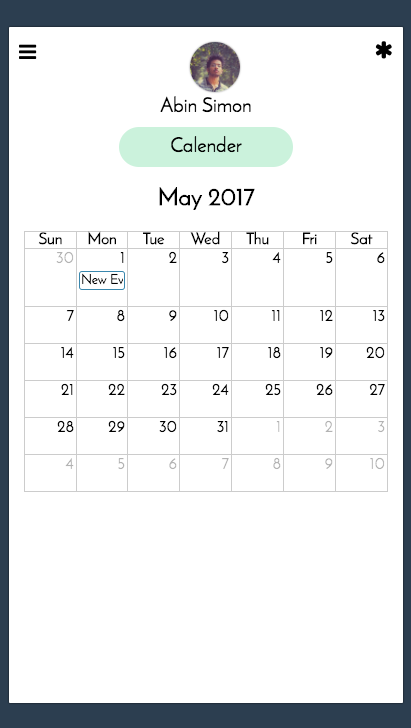
\includegraphics[width=3in]{mobilecalendar.png}
    \caption{Calendar display on mobile}
    \label{fig:mobilecalendar} % insert suitable label, this is used to refer to a fig from within the text as shown above
\end{figure}


\chapter{System Testing}

The aim of the system testing process was to determine all defects in our project. The program was subjected to a set of test inputs and various observations were made and based on these observations it will be decided whether the program behaves as expected or not.

Our Project went through four levels of testing
\begin{itemize}
\item Unit testing
\item Integration testing
\item System testing
\item Component Interface Testing
\end{itemize}

\section{Unit testing}
Unit testing is undertaken when a module has been created and successfully reviewed. In order to test a single module we need to provide a complete en- vironment i.e. besides the module we would require. The procedures which belong to other modules that the module under test calls non local data structures that module access a procedure to call the functions of the mod- ule under test with appropriate parameters. Unit testing was done on each and every module that is described under module wise description.

\section{Integration testing}
In this type of testing we test various integration of the project module by providing the input. The primary objective is to test the module interfaces in order to ensure that no errors are occurring when one module invokes the other module.

\section{System testing}
System testing, or end-to-end testing, tests a completely integrated system to verify that it meets its requirements. For example, a system test might involve testing a logon interface, then creating and editing an entry, plus sending or printing results, followed by summary processing or deletion (or archiving) of entries, then logoff.
In addition, the software testing should ensure that the program, as well as working as expected, does not also destroy or partially corrupt its operating environment or cause other processes within that environment to become inoperative (this includes not corrupting shared memory, not consuming or locking up excessive resources and leaving any parallel processes unharmed by its presence).

\section{Component interface testing}
The practice of component interface testing can be used to check the handling of data passed between various units, or subsystem components, beyond full integration testing between those units. The data being passed can be con- sidered as ”message packets” and the range or data types can be checked, for data generated from one unit, and tested for validity before being passed into another unit. One option for interface testing is to keep a separate log file of data items being passed, often with a timestamp logged to allow analysis of thousands of cases of data passed between units for days or weeks. Tests can include checking the handling of some extreme data values while other interface variables are passed as normal values. Unusual data values in an interface can help explain unexpected performance in the next unit. Com- ponent interface testing is a variation of black box testing, with the focus on the data values beyond just the related actions of a subsystem component.


\chapter{Future Scope}

The project serves all its present requirements. Like any other sys- tem, there is always room for improvement.
The  system in the future expects to be more in every way. Automate more components and also create new components for both teachers and students alike.

\chapter{Conclusion}

A conscious effort has been made while creating and developing the software package ,making use of existing tools, techniques and resource that would cater the demands .The project has shown us the finer aspect of database management system.
While making the system, an eye has been kept on making it as user-friendly, as cost-effective as possible. As such one may hope that the system will be acceptable to any user and will adequately meet his/her needs. The entire project is menu assisted and highly interactive. On trial run the performance was found to be satisfactory. But as in case of any system development processes , there were are a number of shortcomings, there have been some shortcomings in the development of this system also. Thus project is still under modification.

\cleardoublepage
%\pagebreak
\phantomsection
\addcontentsline{toc}{chapter}{References}
\begin{thebibliography}{99}

\bibitem{}Learn python the hard way,\ \url{https://learnpythonthehardway.org/}
\bibitem{}Django official docs,\ \url{https://docs.djangoproject.com/en/1.11/}
\bibitem{}Django Girls Tutorial,\ \url{https://tutorial.djangogirls.org/en/index.html}
\bibitem{}W3 Schools,\ \url{https://www.w3schools.com/}
\bibitem{}Tutorials point,\ \url{https://www.tutorialspoint.com/}
\bibitem{}Stack Overflow,\ \url{http://stackoverflow.com/}
\bibitem{}Udacity,\ \url{https://in.udacity.com/}
\bibitem{}Coursera,\ \url{https://www.coursera.org/}

\end{thebibliography}


\end{document}
